\section{Overall Reflector Blocking}
\label{sec:perfect-blocking}

% Although rather extensive,
Our methodology provides the basis for performing blacklist blocking
measurements at scale: a measurement technique to confidently
determine whether a reflector is blocking a particular IP address, a
viable set of reflectors that are compatible with the technique, and a
set of public security-related blacklists that provide a large set of
candidate IPs that hosts might block.  In this section we describe our
large-scale experiment that uses this methodology for determining
which reflectors block IPs on the public blacklists, and which IPs
they block.  We then present the overall results of the blocking
behavior of reflectors, and subsequent sections explore the different
behaviors in more detail.

%% In this section, we describe in detail our measurement result for the
%% top {\blacklistnum} IP blacklists we picked. In the previous section,
%% we only sampled 5 IPs from each blacklist during the experiment, but
%% now to confidently infer the exact hosts that use each blacklist, we
%% need to increase our sample size.

% \subsection{Experiment Design}

%% In this experiment, we sample 25 IPs from each blacklist, and ensure these
%% sampled IPs satisfy all the requirements listed in
%% Section~\ref{sec:methodology}: exclusive, stable, routable, geo-diversified
%% and not from the {\reflectors}' network. Then we test all the {\reflroughnum}
%% {\reflectors} against 250 blacklist IPs we sampled from all 10 blacklists.
%% Furthermore, to ensure the measurement results are accurate, we include a
%% control group during the experiment by randomly select 20 IPs in United
%% States. These 20 IPs are checked against all the public IP blacklists we have
%% to make sure they are not overlapped with any of the blacklist, and we also
%% ensure these IPs are routable and not from the target hosts' ASes. The
%% control group is constructed that these IPs are unlikely to be all blocked by
%% a {\reflector}, so we eliminate the {\reflectors} that show blocking behavior
%% on more than half of the control IPs.

\begin{figure}[t]
\centering
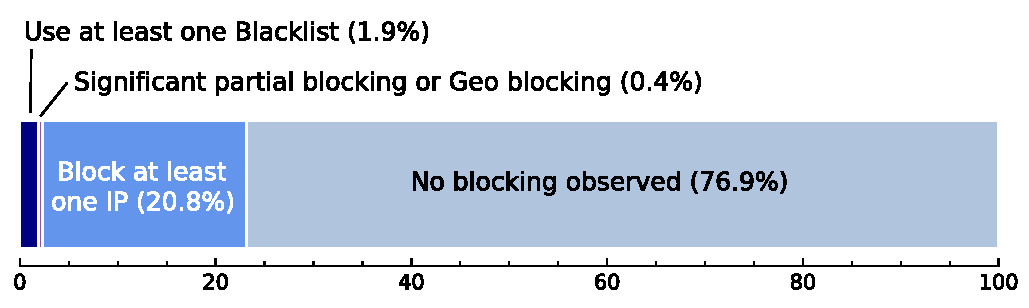
\includegraphics[width=0.95\columnwidth]{images/reflector_breakdown_v2.pdf}
\caption{Breakdown of {\reflector} blocking based on three
  experimental runs.  We identified 4,253 {\reflectors} that use at
  least one blacklist (Section~\ref{sec:blacklist-use}).  We also
  discovered reflectors that block a significant fraction of blacklist
  IPs, due in part to geo-blocking
  (Section~\ref{sec:partial-blocking}).  Finally, we identified a
  large number of reflectors blocking at least one IP, suggesting
  wider use of a much larger set of blacklists
  (Section~\ref{sec:large-scale}).}
\label{fig:reflector-breakdown}
\end{figure}

For a particular experimental run, we randomly selected 25 IPs from
each blacklist that satisfies the requirements defined in
Section~\ref{sec:methodology}: exclusive, stable, routable,
geo-diversified, and AS disjoint. Then we evaluated the blocking
behavior for all {\reflroughnum} {\reflectors} against the 225
blacklist IPs sampled from all nine blacklists. To increase the chances
that these sampled IP will be stable, also to handle cases where reflectors
might update the blacklists slowly(a reflector might take a long time to
start blocking the newest IPs in a blacklist, although we discover
later that it is not the case, see Section~\ref{sec:latency-analysis}),
we ensure the sampled IPs have stayed in the blacklist for at least
2 weeks before our experiment. Since for each blacklist,
an experimental run can takes days to perform, as a post-processing step
we remove blacklist IPs from consideration that did not remain on the
blacklist for the duration of the experiment.

%% After the measurement experiment, we calculate the stable part of the
%% sampled blacklist IPs---IPs that stayed in the blacklist throughout
%% the experiment period, and focus our analysis only on these stable
%% blacklist IPs. We consider a {\reflector} is potentially using a
%% blacklist if the experiment shows it blocked all the stable IPs from
%% that blacklist.

%% we conclude that a {\reflector} is using a blacklist if the experiment
%% shows that it blocked all of these stable IPs from that blacklist.

To increase the amount of evidence of blacklist blocking behavior, we
conducted three experimental runs, each time using a different set of 25
IPs from each blacklist.
%% The first two times we tested against our entire {\reflector} pool,
%% and the third time we tested those {\reflectors} that previously
%% showed block behavior.  \noteby{GV}{Strictly speaking, does this
%%   matter considering how we define blacklist use?}
We then conclude that a {\reflector} is using a blacklist if only if
all experiment runs show that it blocked all the sampled stable IPs
from that blacklist.
%\noteby{VL}{Mention the two week stable thing}.

%In the first
%experiment, we test all the {\reflroughnum} {\reflectors} against the 250 blacklist IPs,
%plus the control IPs. Later, we select the {\reflectors} that had shown at least
%one blocking case, then sample another different set of 25 IPs from each
%blacklist, under our constraints, and conduct the experiment again. We conclude
%a {\reflector} is using a blacklist only if both experiment show it had blocked
%all the sampled stable IPs from that blacklist.

% \subsection{Overall Blocking Behavior}

We conducted our measurements from December 3--23rd, 2019.  During
this period, we tested 96,067,051 distinct \texttt{\small
  ({\reflector},IP)} pairs\footnote{The first two experiment we tested against
  all {\reflectors}, the last experiment we only tested against the ones that
  have shown blocking behavior in the first two tests}.
Based upon the criteria from
Section~\ref{sec:methodology}, we are able to conclusively determine
the blocking behavior (blocking or not blocking) of 98.3\% of the
tested pairs.  Among these pairs, 894,570 pairs display a
clear signal indicating ``blocking''.

Figure~\ref{fig:reflector-breakdown} presents the blocking behavior of
all 222,782 reflectors we tested partitioned into four categories:
those reflectors that we conclude use at least one of the public
blacklists (1.9\%), reflectors that block a large fraction of IPs on
at least one blacklist in every experiment(0.4\%, see more in
Section~\ref{sec:partial-blocking}), remaining reflectors that block at
least one blacklist IP (20.8\%), and reflectors that do not block any
blacklist IPs (76.9\%).  Note that given the requirements for hosts to
be reflectors, such as running old OS versions, it is not surprising a
large percentage shows no blocking of the blacklist IPs: they already
have attributes anti-correlated with high degrees of security hygiene.
Consequently, we want to emphasize that one should not conclude that
this percentage is representative of all hosts on the Internet.

%% Based upon the probing methodology, we conclude that NN {\reflectors}
%% use at least one of the public blacklists we study.

These high-level results provide the foundation for additional
analyses and experiments, and going forward we further investigate
each of these categories of reflector blocking behavior in turn.
Section~\ref{sec:blacklist-use} explores blacklist use among the
{\reflectors}, Section~\ref{sec:partial-blocking} then examines
significant partial blocking behavior (including geo-blocking), and
Section~\ref{sec:large-scale} explores how reflectors that show any
blocking behavior can be used as evidence of much broader use of
blacklists.  As a final analysis, Section~\ref{sec:consistency}
studies the consistency of reflector blocking behavior at a coarser
granularity.

\begin{table}
\setlength{\tabcolsep}{4pt}
\centering
\small
\begin{tabular}{l r r r}
 \toprule
 \textbf{Blacklist} (abbr.)   & \textbf{Reflectors}  & \textbf{/24s}   & \textbf{ASes}\\
 \midrule
 {\spamhausdrop} (DROP)                  & 4,142         & 1,782  & 50  \\
 {\spamhausedrop} (eDROP)                & 1,272         & 362    & 25  \\
 {\dshieldtop} (DTop)                    & 223           & 69     & 18  \\
 {\etcompromised} (ET)                   & 116           & 58     & 15  \\
 {\bdsatif} (BDS)                        & 85            & 41     & 3   \\
 {\feodo} (Feodo)                        & 64            & 26     & 16  \\
 %\textbf{\ciarmy}                              & 59            & 39 \\
 {\snortfilter} (Snort)                  & 52            & 20     & 11  \\
 {\blocklistde} (DE)                     & 36            & 18     & 8   \\
 {\ettor} (Tor)                          & 24            & 9      & 8   \\
 \midrule
 \textbf{Total Unique}                   & 4,253         & 1,827  & 77  \\
 \bottomrule
\end{tabular}
\caption{The number of {\reflectors} we conclude using each of the nine different
  blacklists, as well as the number of unique /24s and ASes those
  reflectors appear in.}
\label{tab:perfect-blocking-reflectors}
\end{table}

\section{Reflectors Using Blacklists}
\label{sec:blacklist-use}

% heatmap
%\begin{figure}[t]
%\centering
%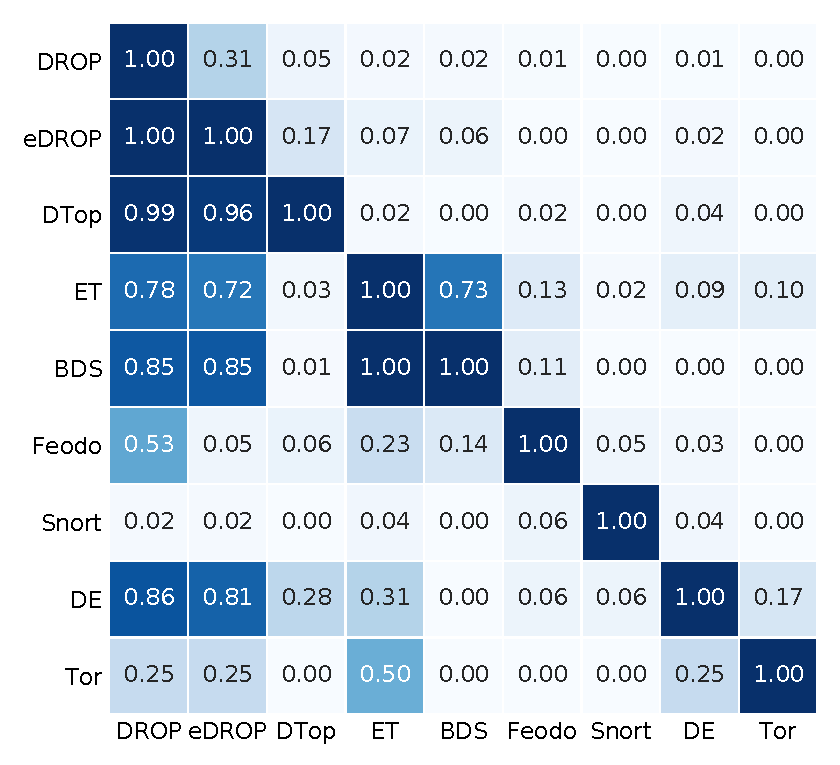
\includegraphics[width=0.85\columnwidth]{images/perfect_blocking_heatmap.pdf}
%\caption{}
%\label{fig:perfect-heatmap}
%\end{figure}
% CDF

%% \begin{figure*}[t!]
%% \begin{subfigure}[t]{0.33\textwidth}
%% 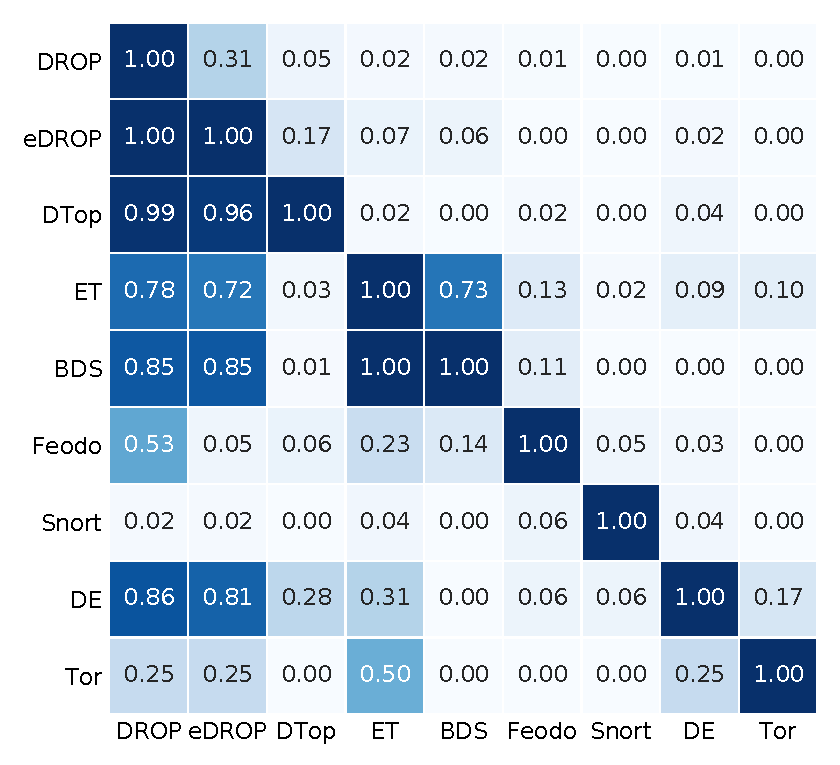
\includegraphics[width=\linewidth]{images/perfect_blocking_heatmap.pdf}
%% \caption{Pair wise intersection between {\reflectors} that use each blacklists}
%% \label{fig:perfect-heatmap}
%% \end{subfigure} %\hspace*{\fill}
%% ~
%% \begin{subfigure}[t]{0.33\textwidth}
%% 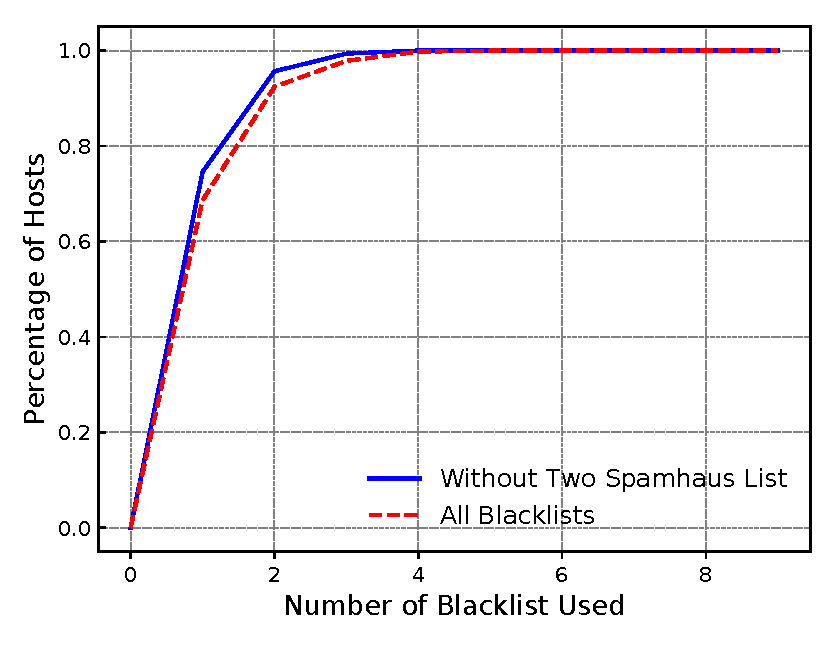
\includegraphics[width=\linewidth]{images/perfect_shared_cdf.pdf}
%% \caption{CDF of the number of blacklists used by {\reflectors}}
%% \label{fig:perfect-shared-cdf}
%% \end{subfigure} %\hspace*{\fill}
%% ~
%% \begin{subfigure}[t]{0.33\textwidth}
%% 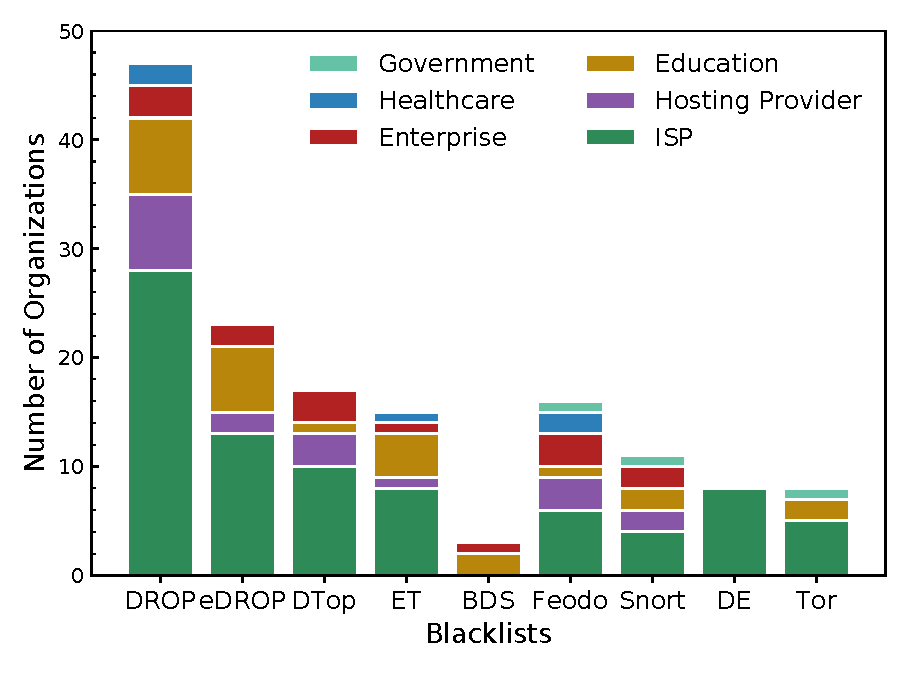
\includegraphics[width=\linewidth]{images/perfect_org_breakdown.pdf}
%% \caption{Breakdown of the organizations covered by each blacklist.}
%% \label{fig:perfect-org-breakdown}

%% \end{subfigure}
%% \end{figure*}

%% \begin{figure}[t]
%%   \centering
%%   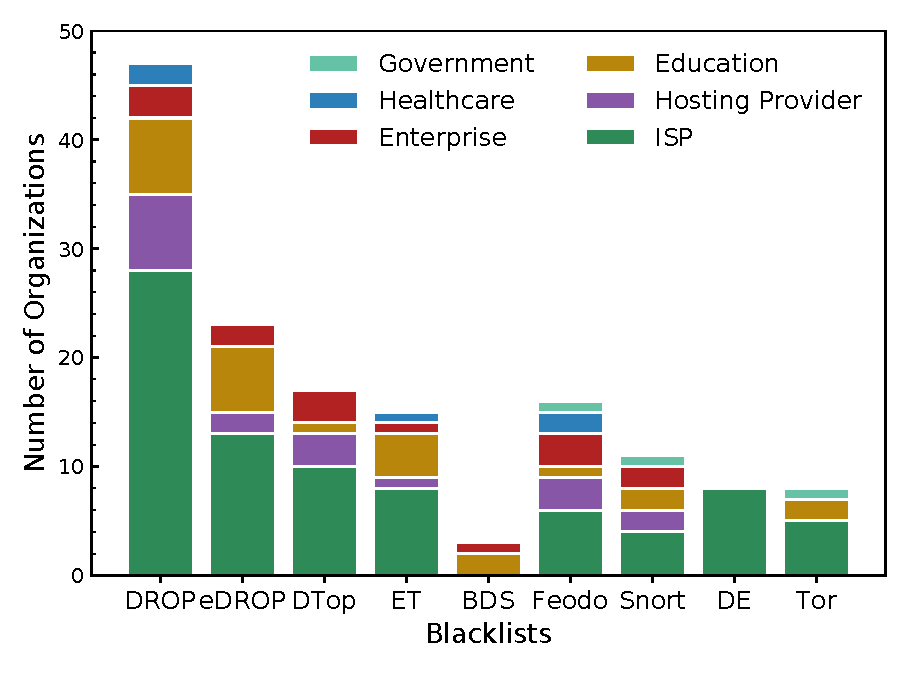
\includegraphics[width=0.85\linewidth]{images/perfect_org_breakdown.pdf}
%%   \caption{Breakdown of the organizations covered by each blacklist.}
%%   \label{fig:perfect-org-breakdown}
%% \end{figure}

%% From Table~\ref{tab:perfect-blocking-reflectors} we can see the number of
%% {\reflectors} that use a particular blacklist is not large.

In this section, we focus on the reflectors that use the blacklists we
study, including the relative popularity of the blacklists, patterns
in the use of multiple blacklists, and the rate at which reflectors
update.  We also use external sources of ground truth to validate our
findings.  Overall, we conclude from the results in this section that
our methodology is indeed effective at identifying blacklist use from
a remote third-party vantage point.

Recall that we use three experimental runs that test whether
reflectors block 25 randomly chosen IPs from the blacklists, and only
conclude that a reflector uses a blacklist if it blocks {\em all}
stable IPs on that blacklist across all runs.  Based on these criteria,
we identified 4,253 reflectors that use one of these public
blacklists.  Table~\ref{tab:perfect-blocking-reflectors} shows the
number of {\reflectors} using each of the nine different blacklists,
as well as the number of unique /24s and ASes those reflectors appear
in.

{\spamhausdrop} is by far the most popular blacklist in our
collection, followed by {\spamhausedrop}.  The remaining blacklists
have a comparatively small number of {\reflectors} using them.  On one
hand, since many aspects of our methodology and experiment make
conservative choices, these results should be considered a lower
bound.  On the other, we have very high confidence in these results:
we believe these reflectors are actually on networks that block the
IPs on these blacklists.

%% These are the only two blacklists that we see over 1,000
%% {\reflectors} using.

%% Figure~\ref{fig:perfect-heatmap} shows the overlap between {\reflectors} that
%% are using each blacklist. At a high level, we can see that hosts using
%% different blacklists overlap significantly with each other. More than 30\% of
%% the {\reflectors} use more than one blacklist.
%% Figure~\ref{fig:perfect-shared-cdf}, shows that if a host uses blacklists, it
%% is likely that it is uses more than one of them. \noteby{GV}{I don't think it does show this?}  Furthermore, {all
%% \reflectors} that use {\spamhausedrop} also use {\spamhausdrop}, which
%% matches our expectation since EDROP list is the extension of DROP list.
%% {\reflectors} that are use {\spamhausdrop} also show significant overlap with
%% multiple other blacklists, indicating {\spamhausdrop} is a popular blacklist,
%% and that if a {\reflector} blocks traffic using blacklists, it would very
%% likely include {\spamhausdrop}.

%% Another important aspect -- the main reason we started looking into this
%% problem -- is to look at the organizations to which the {\reflectors} belong
%% to. However, it is challenging to infer the actual organizations behind these
%% IPs, since at times the most information we can gain from these IPs is the AS
%% organization that announces the IP prefix or the organization listed in the
%% IP WHOIS record. Finally, we decided on using the the CAIDA AS to Organization
%% dataset~\cite{caida_as_org} to map every IP to an organization. We then
%% manually categorize the organizations into six categories: ISPs (service
%% provider like Comcast), Hosting Providers (including web hosting like
%% Godaddy, and cloud providers like Amazon), Education (Universities or
%% schools), Healthcare (Hospitals), Government (Government departments), and
%% Enterprise (Individual companies that owned the registered IPs).
%% Figure~\ref{fig:perfect-org-breakdown} shows the breakdown of the
%% organization categories that show blocking behavior for each blacklist.

%% We can see from the figure that most blacklists are used by a wide category of
%% organizations. {\feodo} has the highest diversity where it covered all six
%% categories we defined, showing that malware threat is under concern by a wide
%% variety of people. If we look from the perspective of organizations, we can see
%% that education institutions have covered 8 of the 9 blacklists we selected,
%% indicating the high impact these blacklists could have on university networks.

%% While Table~\ref{tab:perfect-blocking-reflectors} shows the relative
%% popularity of blacklists, it does not provide insight into how many
%% blacklists a particular organization uses.

%% We now examine blacklist use from the perspective of the organizations
%% that use them.

\begin{figure}[t]
  \centering
  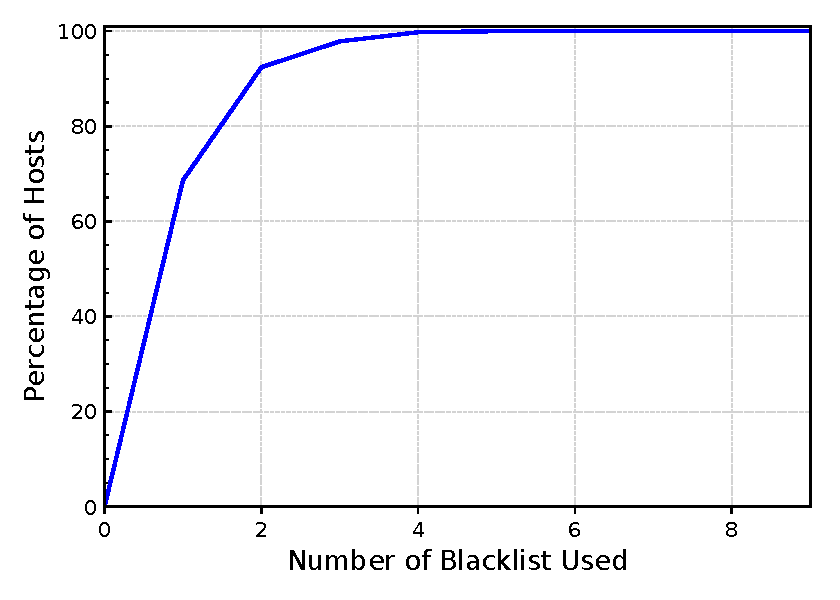
\includegraphics[width=0.8\linewidth]{images/perfect_shared_cdf_v2.pdf}
  \caption{CDF of the number of blacklists used by {\reflectors}}
%%    \noteby{VG}{we should remove this figure}
%%    \noteby{GV}{My vote is to keep it...I think it usefully sets up the heatmap.}
  \label{fig:perfect-shared-cdf}
\end{figure}

\subsection{Multiple Blacklist Use}

For the {\reflectors} using at least one blacklist,
Figure~\ref{fig:perfect-shared-cdf} shows the cumulative distribution
of the number of blacklists they use.  At least for the most popular
public blacklists we study, most use just one.  Over 68.6\% use just
one blacklist, 23.8\% use two or more, and only 7.6\% use three or more.
We see one {\reflector} using six of the nine blacklists -- the most
we see in our study.

For these {\reflectors}, though, there are interesting patterns to the
multiple blacklists used.  Figure~\ref{fig:perfect-heatmap} shows the
use of multiple blacklists with a heatmap.  Rows and columns
correspond to blacklists, and each cell of the heatmap shows the
fraction of the {\reflectors} using the blacklist in row $R$ that are
also using the blacklist in column $C$.  For example, the first cell
for {\etcompromised} shows that 78\% of the {\reflectors} that use ET
also use the {\spamhausdrop} blacklist.  Diagonal cells are 1.00 since
they show blacklists compared with themselves.

The first cell of the {\spamhausedrop} row indicates that all
{\reflectors} that use {\spamhausedrop} also use {\spamhausdrop}.
Since the eDROP list is an extension of the DROP list, the behavior is
strongly consistent with expectations (and, as such, is also a minor
validation of the methodology).  Moreover, the many significant values
in the first two columns show that {\reflectors} that use any of the
other blacklists very often also use {\spamhausdrop} and eDROP.  These
results underscore the popularity of {\spamhausdrop}, and indicate
that if a {\reflector} blocks traffic using blacklists, it very likely
uses {\spamhausdrop}.

%% \noteby{GV}{Note that there is a transition in the granularity in
%%   which we are presenting results, going from {\reflectors} in
%%   Figures~\ref{fig:perfect-shared-cdf} and~\ref{fig:perfect-heatmap}
%%   to the organizations in which those reflectors reside in
%%   Figure~\ref{fig:perfect-org-breakdown}.  Options are: (1) keep as
%%   is, (2) backprop the organization perspective for the CDF and
%%   heatmap graphs, (3) move this to another section.  Since the
%%   behavior of organizations does seem more interesting than individual
%%   {\reflectors}, option (2) is tempting.  How confident are we in the
%%   organization mappings?  And how do these organization mappings
%%   compare/contrast to the /24 consistency results presented later?
%%   Should we also evaluate consistency at the organization
%%   granularity?}

%% Ultimately the blacklist use and blocking behavior of the
%% {\reflectors} is strongly tied to the organization in which they
%% belong.  To explore organizational aspects of blacklist use, we first
%% identify the AS of every {\reflector} that uses a blacklist.  We then
%% use the CAIDA AS-to-Organization dataset~\cite{caida_as_org} to map
%% the AS to an organization, and manually partition the organizations
%% into six categories: ISPs (e.g., Comcast), Hosting Providers (e.g.,
%% GoDaddy web hosting, AWS cloud computing), Education (e.g.,
%% universities), Healthcare (e.g., hospitals), Government (e.g., state
%% and federal agencies), and Enterprise (individual companies owning the
%% IPs).

%% Figure~\ref{fig:perfect-org-breakdown} shows the number of
%% organizations using each blacklist, and their breakdowns by
%% organization category.  The breakdowns indicate that most blacklists
%% are used by a wide variety of organizations.  {\feodo} is the most
%% diverse.  Organizations from all six of our categories use it,
%% emphasizing how malware is a threat of universal concern.
%% {\blocklistde}, in contrast, is used just by ISPs.  \noteby{GV}{Any
%%   ideas why?  What's the nature of DE?}  \noteby{GV}{Also, BDS just
%%   appears in Education and Enterprise, anything about it that would
%%   suggest this result?}

%% If we look from the perspective of organizations, we can see that
%% education institutions have covered 8 of the 9 blacklists we selected,
%% indicating the high impact these blacklists could have on university
%% networks. \noteby{GV}{well, both Education and ISP use 8, and Enterprise
%%   is 7...maybe the following?}  From the other perspective, nearly all
%% of the blacklists are used by Education, ISP, and Enterprise
%% organizations.  In contrast, Healthcare and Government organizations
%% focus on a subset of the lists that...\noteby{GV}{any common theme?}.

%\begin{figure}[t]
%\centering
%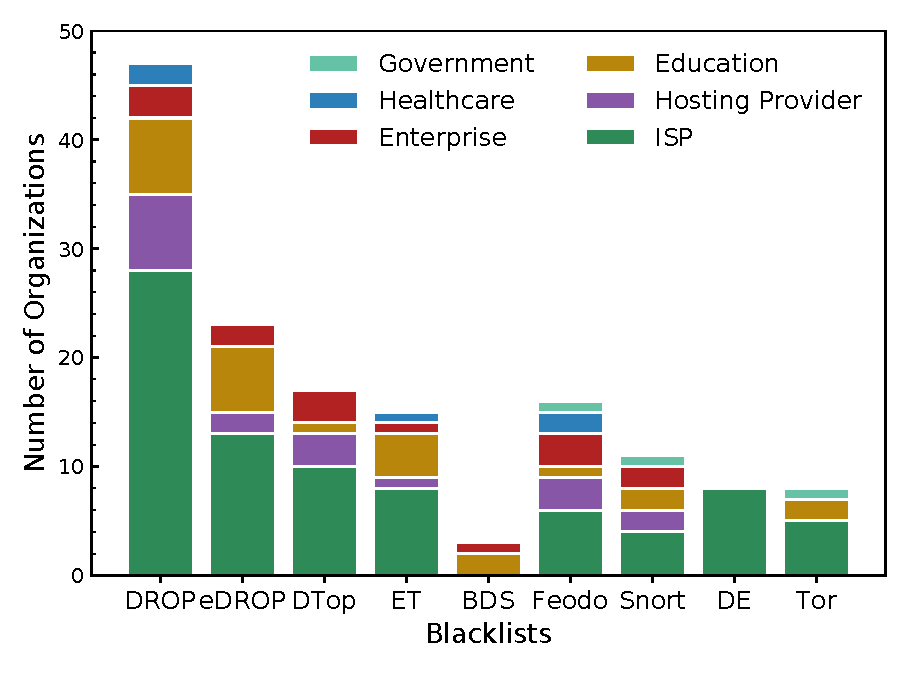
\includegraphics[width=0.85\columnwidth]{images/perfect_org_breakdown.pdf}
%\caption{}
%\label{fig:perfect-org-breakdown}
%\end{figure}

\begin{figure}[t]
  \centering
  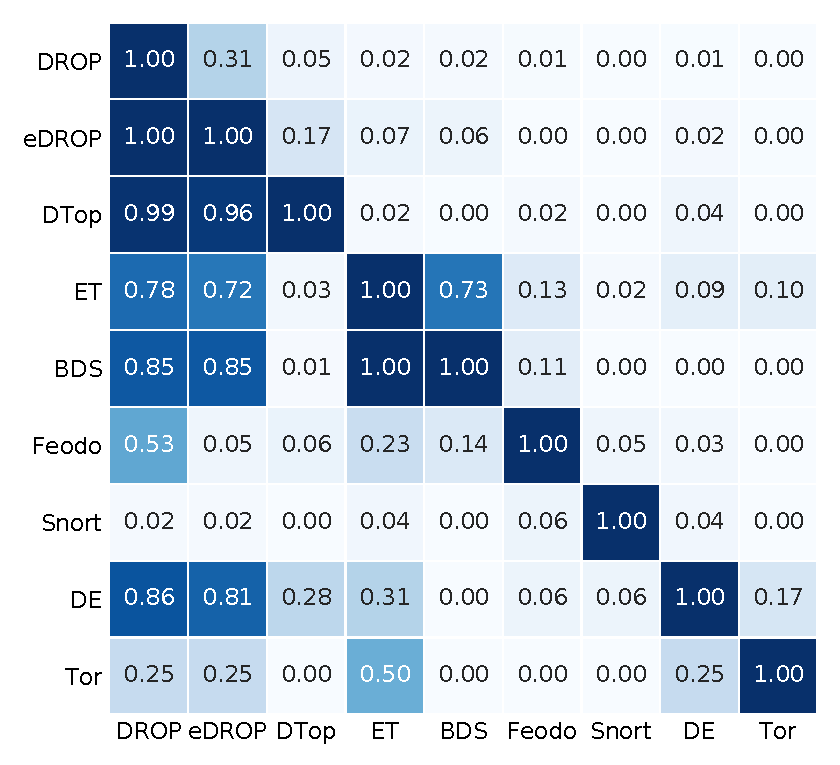
\includegraphics[width=0.85\linewidth]{images/perfect_blocking_heatmap.pdf}
  \caption{Pair-wise overlap of {\reflectors} using the different blacklists.
   Each cell shows the fraction of the {\reflectors} using the blacklist in the
   row $R$ that are also using the blacklist in the column $C$: $|R \cap C| / |R|$.}
  \label{fig:perfect-heatmap}
\end{figure}
